\documentclass{article}
\usepackage[utf8]{inputenc}
\usepackage[english]{babel}
\usepackage{graphicx}
\usepackage{amsfonts}
\usepackage{amsmath}
\usepackage[a4paper, total={7in, 10in}]{geometry}
\newtheorem{theorem}{Theorem}
\newtheorem{definition}{Definition}

\linespread{0.2}

\begin{document}
\section{measure theory}
  
\begin{definition}[Sigma Algebra]
  $\mathcal F$ $\sigma$-algebra:
  \begin{itemize}
  \item $\Omega \in \mathcal F$
  \item $A \in \mathcal F \Rightarrow A^c \in \mathcal F$
  \item $\cup_n A_n \in \mathcal F$
  \end{itemize}
\end{definition}
\begin{definition}[Probability measure]
  Probability measure
  \begin{itemize}
  \item $\mathbb P(A) \in [0, 1]$
  \item $\mathbb P(\Omega) = 1$
  \item $A \cap B = \emptyset \rightarrow \mathbb P(A \cup B) = \mathbb P(A) + \mathbb P(B)$
  \end{itemize}
\end{definition}
\begin{theorem}[Equivalence additive measure]
  The following are equivalent fo $\mu$ finitely additive measure:
  \begin{itemize}
  \item $\mu \sigma-$ additive
  \item $\mu$ continuous from below / above/ at 0.
  \end{itemize}
\end{theorem}
\begin{definition}[Monotone class theorem]
  Monotne class $\mathcal M \subset \mathcal P(\Omega)$,  and is closed under countable monotone unions and intersections.
\end{definition}
\begin{theorem}[Monote class theorem]
  $G$ an algebra, $\sigma(G) = M(G)$
\end{theorem}
\begin{theorem}[$\lambda-\pi$]
  $D$ is a Dynkin system if:
  \begin{itemize}
  \item $\Omega \in D$
  \item $A \in D \Rightarrow A^c \in D$ 
  \item $A_1, \ldots \in D$ pariwise disjoint, $\cup A_i \in D$
  \end{itemize}
  Equivalently
  \begin{itemize}
  \item $\Omega \in D$
  \item $A,B \in D ; A \subset B \Rightarrow B \setminus A \in D$ 
  \item $A_1, \ldots \in D$ increasing, $\cup A_i \in D$
  \end{itemize}

  $P \pi$-system: closed under finite interesection.

  $P \subset D \Rightarrow \sigma(P) \subset P$
\end{theorem}
\begin{theorem}[Sigma in out]
  $$\sigma(f^{-1}(A): A \in \epsilon) = \{ f^{-1}(A): A \in \sigma(\epsilon) \}$$
\end{theorem}
\begin{definition}[Semi-ring]
  \begin{itemize}
  \item $\emptyset \in S$
  \item $A \cap B \in S \forall A, B \in S$
  \item For al $A, B \in S$ there exist pairwise disjoint subset $C_1, ..., C_n \in S$ such that $A \setminus B = \cup_{i \le n} C_i$
  \end{itemize}
\end{definition}
\begin{theorem}[Caratheodory's Extension Theorem]
  \begin{itemize}
  \item A measure $\mu$ on a semi-ring $S$ can be extendted to a
    measure on $\sigma(S)$.
  \item If $\mu$ is $\sigma$-finite, the extension is unique.
  \end{itemize}
\end{theorem}
\begin{definition}[Consistence]
  \begin{itemize}
  \item $\mathbb P^{i_1, ..., i_n}[A_1 \times ... \times A_n] = \mathbb P^{\pi(i_1), ... , \pi(i_n)}[A_{\pi(1)} \times ... \times A_{\pi(n)}]$
  \item $\mathbb P^{i_1, ..., i_{n-1}}[A_1 \times ... \times A_{n-1}] = \mathbb P^{i_1, ..., i_n}[A_1 \times ... \times A_{n-1} \times \mathbb R] $
  \end{itemize}
\end{definition}
\begin{theorem}[Kolmogorov's Extension Theorem]
  $I$ non empty.
  $(\mathbb P^{i_1, ..., i_n})_{i_1, ..., i_n \in I}$ consistent family. There exists a unique probability measure on $\mathbb P$ on $(\mathbb R^I, \mathbb B(\mathbb R)^{\times I})$ such that
  $$\mathbb P[\{ \omega \in R^I: (\omega_{i_1}, ..., \omega_{i_n}) \in B] = \mathbb P^{i_1, ..., i_n}[B]$$
\end{theorem}

\section{Integrals}
\begin{theorem}[Monotone Convergencen]
  $f_1, \ldots$  be a pointwise non-decreasing sequence of non-negative valued measurable functions, set $\sup f_n = f$. Then $f$ is measurable and
$\lim_{k\to\infty} \int f_k \, \mathrm{d}\mu = \int f \, \mathrm{d}\mu$.
\end{theorem}
\begin{theorem}[Fatou]
  Let $f1, f2, f3, \ldots$ be a sequence of non-negative measurable functions.  Define $f = \liminf_{n\to\infty} f_n$.
Then $f$ is measurable and $\int_S f\,d\mu \le \liminf_n \int_S f_n\,d\mu$.

\end{theorem}
\begin{theorem}[Dominated Convergence]
  $g, f_1, f_2, \ldots$ measurable functions suchat $\int |g| < \infty$, $|f_n| \le g \forall n$ a.s., $f_n \overset{\text{a.s.}}\rightarrow f$, then
  $\int |f| \le \int |g| < \infty$ and $\lim \int |f_n - f| \rightarrow 0$, $\lim \int f_n \rightarrow \int f$
\end{theorem}
\begin{theorem}[Funbini]
  $\mu_1, \mu_2$ are $\sigma$-finite.
  \begin{itemize}
  \item $\int_{\Omega_1 \times \Omega_2} |f| d(\mu_1 \times \mu_2) < \infty \Rightarrow
    \int_{\Omega_1 \times \Omega_2} f d(\mu_1 \times \mu_2)
    = \int_{\Omega_1}\int{\Omega_2} f$
  \item $f \ge 0 \, \text{a.s}\; \Rightarrow
    \int_{\Omega_1 \times \Omega_2} f d(\mu_1 \times \mu_2)
    = \int_{\Omega_1}\int{\Omega_2} f$
  \end{itemize}
\end{theorem}
\begin{theorem}[Inequalities]
  \begin{itemize}
  \item Holder: $ \frac1p + \frac1q = 1 \Rightarrow \int |fg| \le (\int |f|^p)^{\frac 1p}(\int |g|^q)^{\frac 1q}$
  \item Minkowsky: $\forall p \le 0 \; ||f + g||_p \le ||f||_p + ||g||_p$
  \end{itemize}
\end{theorem}
\begin{theorem}[Borel Cantelli]
  \begin{itemize}
  \item $\sum \mathbb P(A_n) < \infty \Rightarrow \mathbb P[\cap_m \cup_{n \ge m} A_n] = 0$
  \item $(A_n) ,\text{indepedent}, \; \sum \mathbb P(A_n) = \infty \Rightarrow \mathbb P[\cap_m \cup_{n \ge m} A_n] = 1$
  \end{itemize}
\end{theorem}

\section{Random Variables}
\begin{definition}[Uniform integrability]
  $(X_i)$ u.i iff $\lim_c \sup_i \int_{|X_i| > c} |X_i|d\mathbb P = 0$
  iff $\lim_n \sup_i \mathbb E[1_{|X_i| > c}|X_i|]  = 0$
\end{definition}
\begin{theorem}[Caracterisation]
  \begin{itemize}
  \item $\forall i |X_i| \le X \in L_1 \Rightarrow (X_i)$ uc
  \item uc iff:
    \begin{itemize}
    \item $\sup E[|X_i|] < \infty$
    \item $\forall \epsilon > 0, \exists \delta > 0 \forall A \mathbb P(A) < \delta \Rightarrow  \forall i \int_A |X_i| < \epsilon$
    \end{itemize}
  \end{itemize}
\end{theorem}
\begin{theorem}[$L_1$ Convergencen]
  $X_i \overset{\mathbb P}{\rightarrow} X$, $X_i$ uc. Then $X \in L_1$, $X_i \overset{L_1}{\rightarrow} X$
  
\end{theorem}
\begin{theorem}[De la Valle-Pousson]
  $X_i$ uc $\iff$ $\exists \Phi: \mathbb R^+ \rightarrow \mathbb R^+,\frac{\Phi(x)}{x}\rightarrow \infty \text{st} \sup E[\Phi |X_i|] < \infty$.
  $\Phi$ can be assumed convex and non-decreasing.
\end{theorem}
\begin{theorem}[Week Law of large numbers]
  $X_i \in L_2$ uncorrelated, $E[X_i] = m, \sup E[X_i^2] < \infty$, then $\frac{\sum_i X_i}{n} \rightarrow m$ in $L_2$.
\end{theorem}
\begin{theorem}[Caracteristic Function]
  \begin{itemize}
  \item $|\Phi_X(u)| < \Phi_X(0) = 1$
  \item $\Phi_X(-u) = \bar {\Phi_X(y)}$
  \item $\Phi_X \in \mathbb R \iff X \overset{\mathbb D}{=} -X$
  \item $\Phi_x$ is unifromly continuous.
  \item $E[|X|^n] < \infty \Rightarrow \exists \Phi^{k}_X \forall k \le n$, and $\Phi_X^k(u) = E[(iX)^ke^{iuX}]$, and $\Phi_X(u) = \sum_k^n \frac{(iu)^k}{k!}E[X^k] + \frac{(iu)^n}{n!}\mathcal E_n(u)$, with $\mathcal E_n \rightarrow_0 0$
  \item $\exists \Phi^{2k}_X(0) \Rightarrow E[X^{2k}] < \infty$
  \item Inversion Formula: $\frac{F_X(b) + F_X(b^-)}{2}- \frac{F_X(a) + F_X(a^-)}{2} = \lim \frac{}{2\pi} \int_{-c}^{c} \frac{e^{-iua} - e^{-iub}}{iu}\Phi_X(u) du$
  \item $\int_R |\Phi_X| < \infty \Rightarrow f_X(x) = \frac{1}{2\pi} \int_{-\infty}^{\infty} e^{iux} \Phi_X(u) du$
  \item $X = (X_1, \ldots X_n)$ indepdendent $\iff \Phi_X = \prod \Phi_{X_i}$
  \end{itemize}
\end{theorem}
\begin{theorem}[Continuity Theorem]
  \begin{itemize}
  \item $X_n \overset{D}{\rightarrow} X \iff \Phi_{X_n} \rightarrow \Phi_X$
  \item $\Phi_{X_n} \rightarrow \Phi$ and $\Phi$ continuous at $0$ then $\exists X \; X_n \overset{D}{\rightarrow} X$
  \item $X_n \overset{D}{\rightarrow} X \iff F_n \overset{\text{in} \; C(F_X)}\rightarrow F_X$
  \end{itemize}
\end{theorem}
\begin{theorem}[LLN]
  $X_i$ iid in $L_1$, $\frac{\sum X_i}{n} \rightarrow E[X]$ as and in $L_1$
\end{theorem}
\begin{theorem}[CLT]
  $X_n$ iid $Var(X) = \sigma^2 < \infty$ then $\frac{1}{\sqrt n}\sum \frac{X_i - E[X]}{\sigma} \rightarrow \mathcal N(0, 1)$
\end{theorem}

\section{Martingales}
\begin{theorem}[Radon-Nikodym]
  $\mu_2 << \mu_1 \Rightarrow \exists f \text{unique $\mu_1$-a.s} \; f = \frac{d\mu_2}{d\mu_1}$
\end{theorem}
\begin{theorem}[Stopping times]
  \begin{itemize}
  \item $X_n^{\tau} = X_0 + (V.X)_n$ is martingale because $V$ is
    predictable.
  \item If $\tau$ bounded $E[X_0] = E[X_{\tau}]$
  \item $M \ge \tau \ge \sigma$ stopping times, then $E[X_{\tau} | F_{\sigma}] = X_{\sigma}$
  \end{itemize}
  
\end{theorem}
\begin{theorem}[Upcrossing inequality]
  $X_n$ submartingale. $E[B_n(a, b)] \le \frac{E[(X_n - a)^+]}{b - a}$
\end{theorem}
\begin{theorem}[Convergence]
  \begin{itemize}
  \item $X_n$ submartingale, $L_1$ bounded, then there exists  $X_{\infty}$ such that  $X_n \overset{a.s}{\rightarrow} X_{\infty}$, and  $E[|X_\infty|] < \sup E[|X_n|]$
  \item a submartingale that is bounded above converges a.s.
  \item $X_n$ ui submartingale, then there exists $X_{\infty} \in L_1$ such that $X_n \rightarrow X_{\infty}$ in $L_1$. Moreover $E[X_{\infty} | F_n] \ge X_n$.
  \item $(F_n)$ filtration, $E[X | F_n] \rightarrow E[X | \cup F_n]$ a.s and $L_1$ (because u.i.)
  \item $X_i$ iid, $\mathcal G = \cup \sigma(X_n, \ldots)$, then $\forall A \in \mathcal G \; P(A) \in \{0, 1\}$ (because $1_A = E[1_A]$)
  \item $(G_i)$ dec-filtration, $E[X | G_n ] \rightarrow E[X | \cap G_n]$ as and in $L_1$.
  \end{itemize}
\end{theorem}
\begin{theorem}[Doob Maximal inequality]
  $X_n$ non-negative submartingale.
  \begin{itemize}
  \item $\forall \lambda > 0$, then $\lambda^p \mathbb P[\max_{k \le n} X_k \ge \lambda] \le E[X_n^p]$
  \item $|\max_{k \le n} X_k|_p \le \frac{p}{p-1} |X_n|_p$
  \item $|\max_{k \le n} X_k|_1 \le \frac{e}{e-1} (1 + |X_n\log(X_n)|_1)$
  \end{itemize}
\end{theorem}
\begin{theorem}[Random Walk]
  \begin{itemize}
  \item Fair random walk, $S_0 = 0, \tau = \inf\{n: S_n\in \{A, -B\} \}$:
    $$P(X_\tau = A) = \frac{B}{A+B}$$
    $$E[\tau] = AB$$
    $$P(\tau < \infty) \ge P(\tau_A < \tau_{-B}) \rightarrow 1$$

  \item $p \ne \frac12$, $P(X_{\tau} = A) = \frac{(\frac{1-p}p)^B - 1}{(\frac{1-p}p)^{A+B} - 1}$,
    \[
      P(\tau_A < \infty) = \lim_B P(\tau_A < \tau_{-B}) =
      \left\{\begin{array}{cc}1&\text{if } p > \frac12\\(\frac{p}{1-p})^A&\text{else}\end{array}\right.
    \]
    \[
      E[\tau_A] = \lim E[\tau_A \wedge \tau_{-B}] =
      \left\{\begin{array}{cc}\frac{A}{2p-1}&\text{if } p > \frac12\\\infty&\text{else}\end{array}\right.
    \]
  \end{itemize}
\end{theorem}

\section{Markov}
\begin{theorem}[Markov property]
  \begin{itemize}
  \item $(X_n)$ markov $(\lambda, P)$. Conditional on $X_m = i$,
    $X_{n+m}$ is markov $(\delta_i, P)$ independent of
    $X_0, ..., X_m$.
  \item $(X_n)$ markov $(\lambda, P)$. Conditional on
    $X_T = i$, $X_{n+T}$ is markov $(\delta_i, P)$ independent of
    $X_0, ..., X_T$.
  \end{itemize}

\end{theorem}
\begin{definition}[Some defs]
  \begin{itemize}
  \item Communicating classes: $I / \sim$ where $i \sim j \iff i \leftrightarrow j$
  \item $C$ Closed $\iff i \in C, i \rightarrow j \Rightarrow j \in C$
  \item $P$ irreducible $\iff \forall i, j, i \rightarrow j \iff $  there is only one communicating class.
  \item $H_i = \inf\{ n \ge 0; X_n = i\}, T_i = \inf\{n \ge 1; X_n = i \}, V_i := \sum_n 1_{\{X_n = i\}}, f_i = P_i(T_i < \infty), m_i = E[T_i]$
  \item $i$ is reccurent if $P_i(V_i = \infty) = 1 \iff f_i = 1 \iff \sum p_{ii}^{(n)} = \infty$, otherwise transient.
  \item $i$ is positibe recurrent $\iff m_i < \infty$ 
  \item $P_i(V_i \ge k + 1) = f_i^k$
  \item In a communcating class all cstates are transient or all are reccurrent.
  \item recurrence $\Rightarrow$ closed
  \item finite  + closed $\Rightarrow$ recurrent.
  \item $P$ irreducible + recurrent $\Rightarrow P(T_j < \infty)$
  \item $i$ aperiodic $\iff p_{ii}^{n} > 0$ for large $n$
  \item $\lambda_i p_{ij} = \lambda_j p_{ji} \Rightarrow \lambda$ is invariant.
  \end{itemize}
\end{definition}
\begin{theorem}[Invariant Distribution]
  \begin{itemize}
  \item $I$ finite, if for some $i \in I$ $p_{ij}^{(n)} \rightarrow \pi_j \forall j \in I$ then $\pi$ is an invariant distribution.
  \item if $P$ irreducible and $\lambda \ge 0$ invariant, then $\lambda \in \{0, \infty, \mathbb R^n\}$
  \item $\gamma_i^k = E_k [\sum^{T_k-1}_{n = 0} 1_{X_n = i}]$.
    If $P$ irreducible and recurrent, then
    \begin{itemize}
    \item $\gamma_k^k = 1$
    \item $\gamma^k$ is invariant
    \item $0 < \gamma^k < \infty$
    \end{itemize}
  \item If $P$ irreducible and $\lambda$ invariant with $\lambda_k = 1$ then $\lambda \ge \gamma^k$. If $P$ is reccurent, $\lambda = \gamma^k$.
  \item If $P$ irreducible, every state is positive recurrent $\iff$ state $i$ is pos rec $\iff$ P has invariant distribution $\pi$. Moreover $\pi_i = 1/m_i$
  \end{itemize}
\end{theorem}
\begin{theorem}[Convergences]
  $P$ transition matrix of an ergodic Markov chain (irreducible, aperiodic and positive recurrent), with invariant measure $\pi$, then for any initial distribution, $P(X_n = j) \rightarrow \pi_j$
\end{theorem}
\begin{theorem}[Ergodic theorem]
  \begin{itemize}
  \item $P$ irreducible, then $\frac{V_n(n)}{n} \rightarrow \frac{1}{m_i}$ as.
    If $P$ is irreducible and positive recurrent, for every bounded function:
    $\frac{1}{n} \sum^{n-1} f(X_k) \rightarrow \sum_i \pi_i f(i)$ a.s 
  \end{itemize}

\end{theorem}
\begin{theorem}[Time reversal]
  $P$ irreducible and have an invariant distribution $\pi$.
  if $X_i \sim Markov(\pi, (P_{ij}))$ then $X_{N-i} \sim Markov(\pi, (P_{ji}))$
\end{theorem}
\begin{theorem}[Coupling theorem]
  $X, Y \sim Markov(\lambda / \pi, P)$ indenpendent, $W_n = (X_n, Y_n) \sim Markov(\lambda \otimes \pi, P \otimes P)$
\end{theorem}


\section{Complex Analysis}


\begin{theorem}[Cauchy]
  Suppose $U$ is an open subset of the complex plane $\mathbb C$,
  $f : U \rightarrow \mathbb C$ is a holomorphic function and the
  closed disk $D = \{ z: |z-z_0| \le r\}$ is completely contained
  in $U$. Let $\gamma$ be the circle forming the boundary of $D$. Then
  for every a in the interior of $D$:
$$f(a) = \frac{1}{2\pi i} \oint_\gamma \frac{f(z)}{z-a}\, dz $$
where the contour integral is taken counter-clockwise.
\end{theorem}

\section{Annexe}
\begin{theorem}[Tower]
\begin{align*}
  E[1_{Y \in B} F(y)] &= \int 1_{y \in B} F(y) f(y) dy\\
                      &= \int 1_{y \in B} (\int 1_{x \le y} f(x)dx) f(y) dy\\
                      &= \int 1_{y \in B}  1_{x \le y} f(x) f(y) dx dy & \text{Tonnelli, positive}\\
                      &= \int 1_{y \in B}  1_{x \le y} dP_{X,Y}\\
                      &= E[1_{Y \in B} 1_{X \le Y}]
\end{align*}
$F(Y)$ is $\sigma(Y)$-measurable.  So
$P(X \le Y | Y ) = E[1_{X \le Y} | Y] = F(Y)$
\end{theorem}

\section{Common distribution}

\[
\begin{array}{l|l|l}
\text{Order}&\text{Non-central moment}&	\text{Central moment}\\
1    &\mu	&0\\
2    &\mu^2  + \sigma^2 &\sigma^  2\\
3    &\mu^3  + 3\mu \sigma^  2&0\\
4    &\mu^4  + 6\mu^2 \sigma^2  + 3\sigma^4 &3\sigma^  4\\
5    &\mu^5  + 10\mu^3 \sigma^2  + 15\mu \sigma^  4&0\\
6    &\mu^6  + 15\mu^4 \sigma^2  + 45\mu^2 \sigma^4  + 15\sigma^6 &15\sigma^  6\\
7    &\mu^7  + 21\mu^5 \sigma^2  + 105\mu^3 \sigma^4  + 105\mu \sigma^  6&0\\
8    &\mu^8  + 28\mu^6 \sigma^2  + 210\mu^4 \sigma^4  + 420\mu^2 \sigma^6  + 105\sigma^8 &105\sigma^  8\\
\end{array}
\]
\begin{figure}
  \centering
  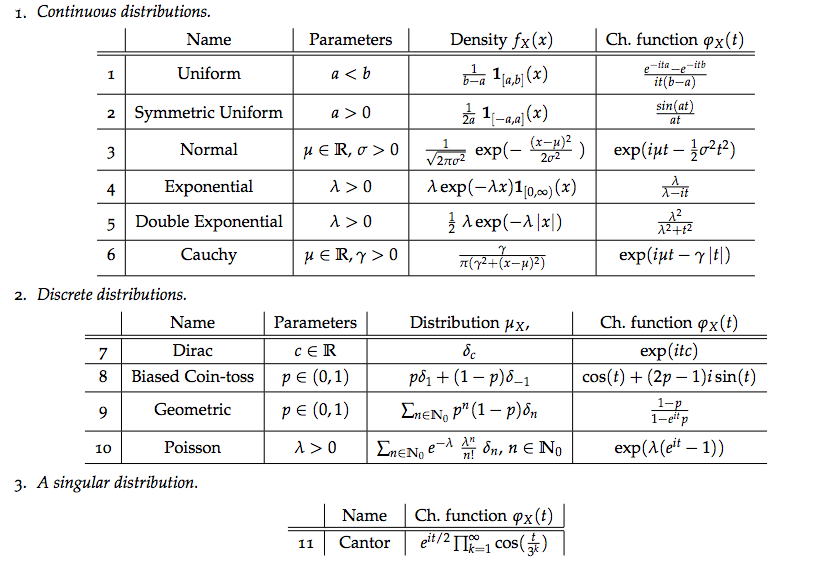
\includegraphics[scale=0.65]{distributions.png}
  
\includegraphics[scale=0.8]{gamma.png}
  \caption{Distributions(gamma mean var)}
\end{figure}


\end{document}

  

























